\chapter*{Task 4}
\addcontentsline{toc}{chapter}{Task 4}

Task 4 requires linearizing the dynamics about the generated optimal trajectory $(x^{star},u^{star})$ and exploiting the MPC algorithm to define a robust control law, able to track the reference trajectory.

Model Predictive Control is a technique that at each time iteration solves the whole optimal control problem for a fixed time window and applies only the first optimal input. After the first iteration, it moves the time window forward and starts computing the next optimal input. For this reason, Model Predictive Control works in an infinite time horizon.

How the optimal control problem is solved at each iteration depends on what cost and dynamics are present. This allows managing constraints directly with the certainty that they will be satisfied.

Since, in this case, constraints are not present, the cost is quadratic and the dynamics are linearized, we can solve the MPC problem by exploiting an LQR solution each time (\ref{MPC}).

The task assignment requires considering an initial perturbed condition different from 0. In addition, we have applied noise inside the control loop like in Task 3.

The control law applies a feedforward action that is the optimal input obtained with Newton's method and then uses the MPC solution to stabilize the system.

\begin{equation} \label{MPC}
    \begin{cases}
        &\\
        &\min_{\Delta x \Delta u} \hspace{0.1cm} \sum_{\tau=t}^{t+T-1} \Delta x_{\tau}^TQ^{reg}\Delta x_{\tau} + \Delta u_{\tau}^TR^{reg}\Delta u_{\tau} + \Delta x_{t+T} ^TQ_T^{reg}\Delta x_{t+T} \\
        &subj. to \hspace{0.5cm} \Delta x_{\tau+1} = A_{\tau} \Delta x_{\tau}  + B_{\tau} \Delta u_{\tau} \\
        & \hspace{2cm} \Delta x_0 =  x_t + n_m \\
        &\\
        &{u}_t = u_t^{mcp} + u_t^{star} + n_a\\
        &{x}_{t+1} = f_d(x_t,u_t)\\
        &
    \end{cases}
\end{equation}

The weights in the regulator cost have been selected as:

\begin{equation*}
    \begin{aligned}
        &Q_t^{mpc} = \begin{bmatrix}
            1000 & 0 & 0 & 0 \\
            0 & 1000 & 0 & 0 \\
            0 & 0 & 10 & 0\\
            0 & 0 & 0 & 10
        \end{bmatrix} = Q_T^{mpc}\\
        &\\
    & R^{mpc}_t = 10
    \end{aligned}
\end{equation*}

The time window we have chosen is 1 second (100 samples). We selected it by trying various values and chose a trade-off between performance and computational time.

As we can see from the plots, the system follows the reference, and the control loop is robust with respect to noise and a perturbed initial condition.

\begin{figure}
    \centering
    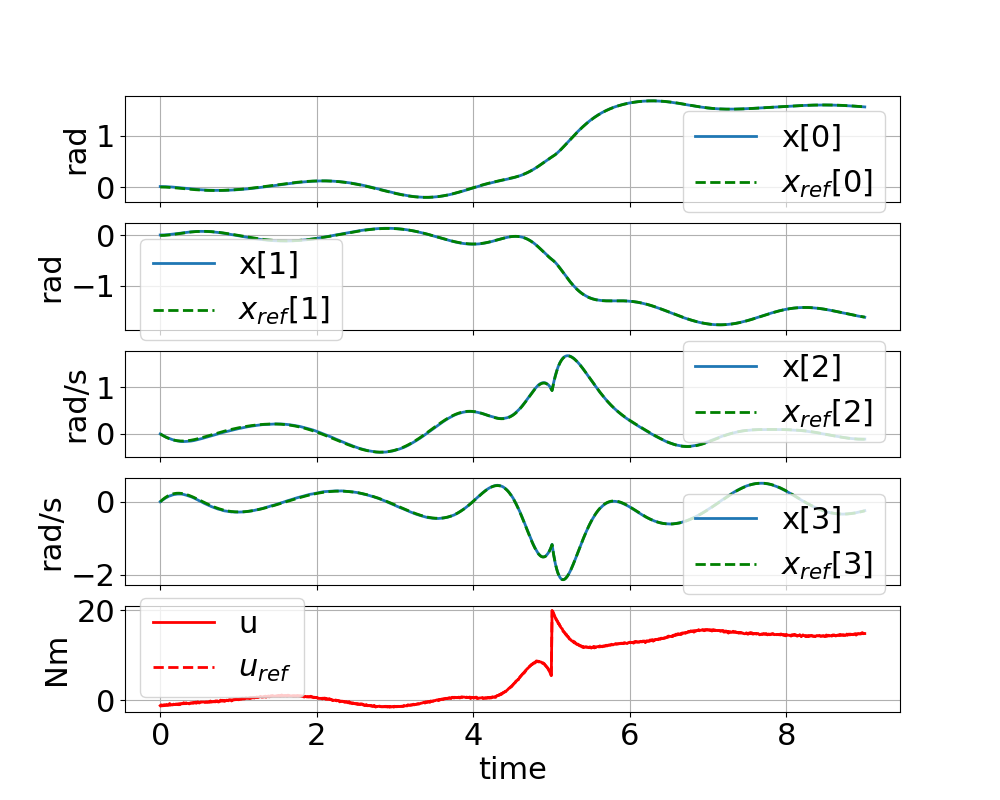
\includegraphics[width=0.8\linewidth]{figs/downward_mpc_track.png}
    \caption{Reference Tracking with MPC}
    \label{fig:downward_mpc_track}
\end{figure}

\begin{figure}
    \centering
    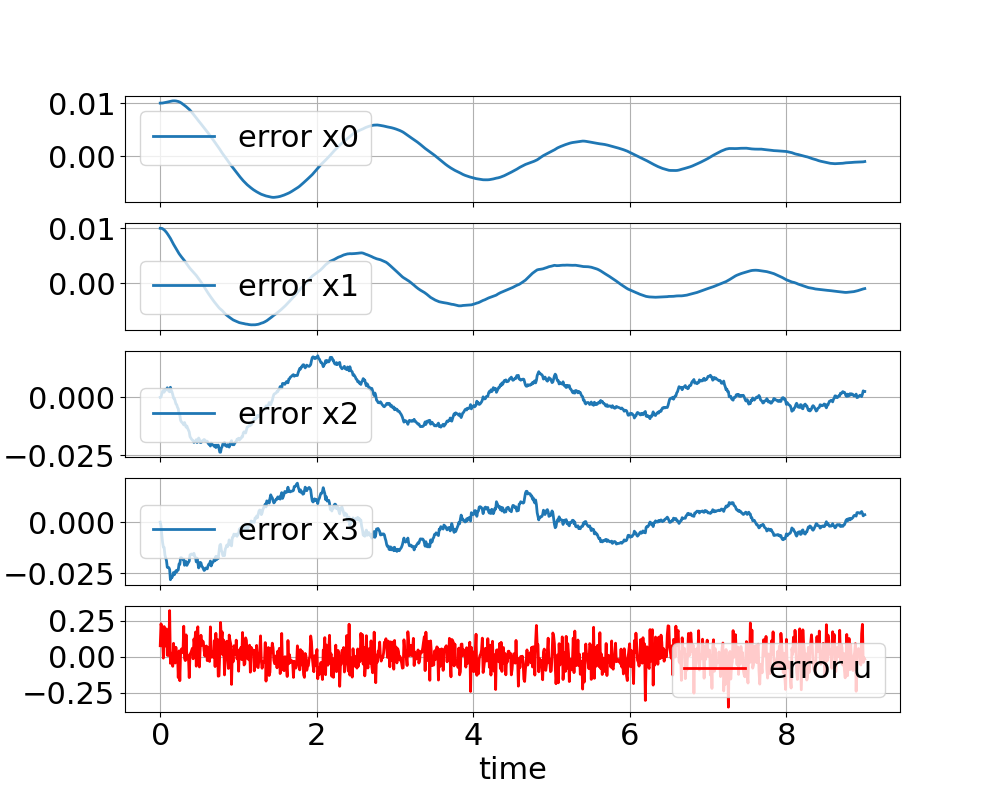
\includegraphics[width=0.8\linewidth]{figs/downward_mpc_error.png}
    \caption{Tracking error}
    \label{fig:downward_mpc_error}
\end{figure}

\begin{figure}
    \centering
    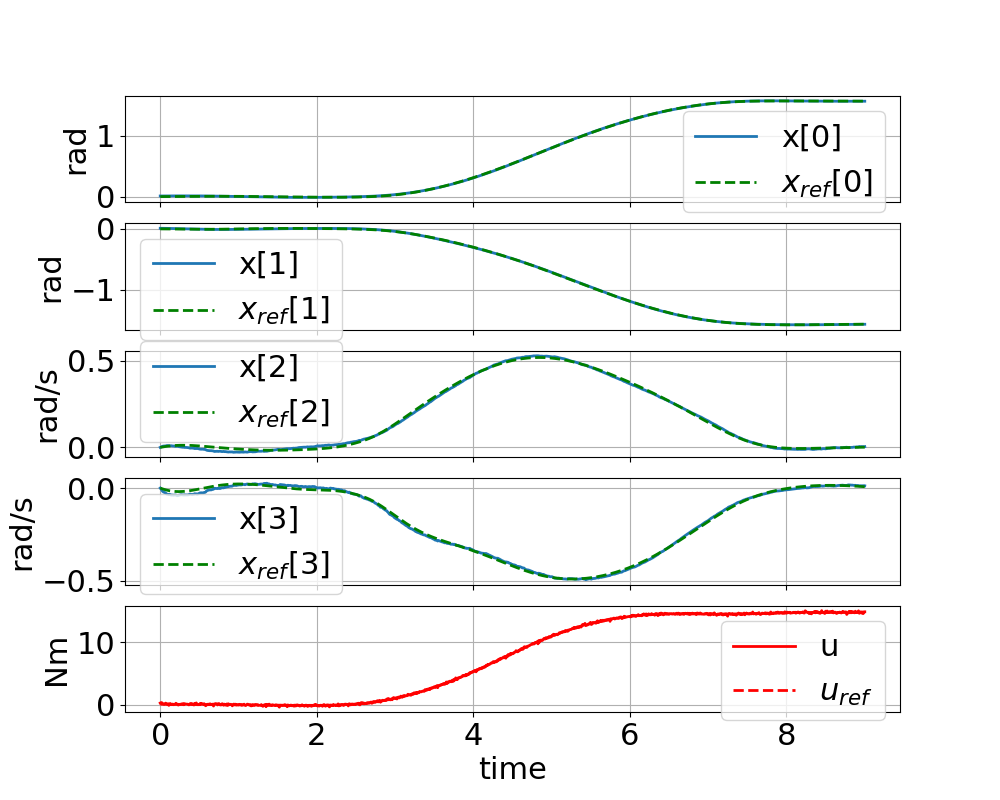
\includegraphics[width=0.8\linewidth]{figs/downward_mpc_track_smooth.png}
    \caption{Smooth reference Tracking with MPC}
    \label{fig:downward_mpc_track_smooth}
\end{figure}

\begin{figure}
    \centering
    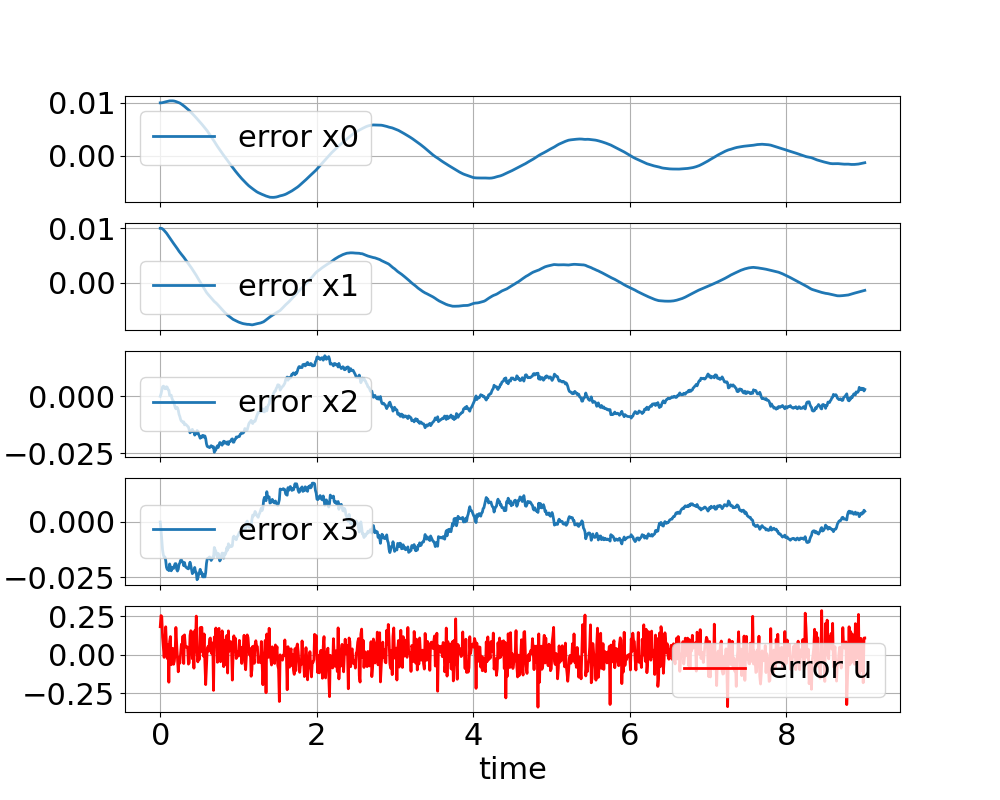
\includegraphics[width=0.8\linewidth]{figs/downward_mpc_error_smooth.png}
    \caption{Smooth reference tracking error}
    \label{fig:downward_mpc_error_smooth}
\end{figure}

\section*{Python code}
The MPC solver is defined in the Python file \texttt{solver.py}. The function calls the LQR function to obtain a gain \( K^* \), and then uses it to compute the optimal input as \( \Delta u_t = K_t \cdot \Delta x_t \).

\begin{itemize}
    \item \textbf{solver\_linear\_mpc(dyn, A\_f, B\_f, QQ, RR, QQf, xx\_t, xx\_star, uu\_star, dt, T\_pred = 20) }: Compute the optimal gain matrix $K_t^*$ for each time instant.\\\\
    \textbf{Arguments}:
    \begin{itemize}
        \item dyn : dynamic package imported from Dinamics.py.
        \item A\_f : Symbolic rappresentation of the discretized state jacobian.
        \item B\_f : Symbolic rappresentation of the discretized input jacobian.
        \item QQ : Weight matrix for the states.
        \item RR: Weight matrix for the inputs.
        \item QQf : Weight matrix for the states at the final time T.
        \item xx\_t : measured input at time t.
        \item xx\_star : Optimal state reference trajectory in the time window.
        \item uu\_star : Optimal input reference trajectory in the time window.
        \item dt : Time of dicretization in seconds.
        \item T\_pred : Time prediction window size in seconds.
    \end{itemize}
    \textbf{Return}:
    \begin{itemize}
        \item uu\_mpc: Optimal input at time t.
    \end{itemize}
\end{itemize}